\subsubsection{UC\theuccount-BT - Consumer Telegram inoltra il messaggio finale al bot Telegram}
	\begin{figure}[H]
		\centering
		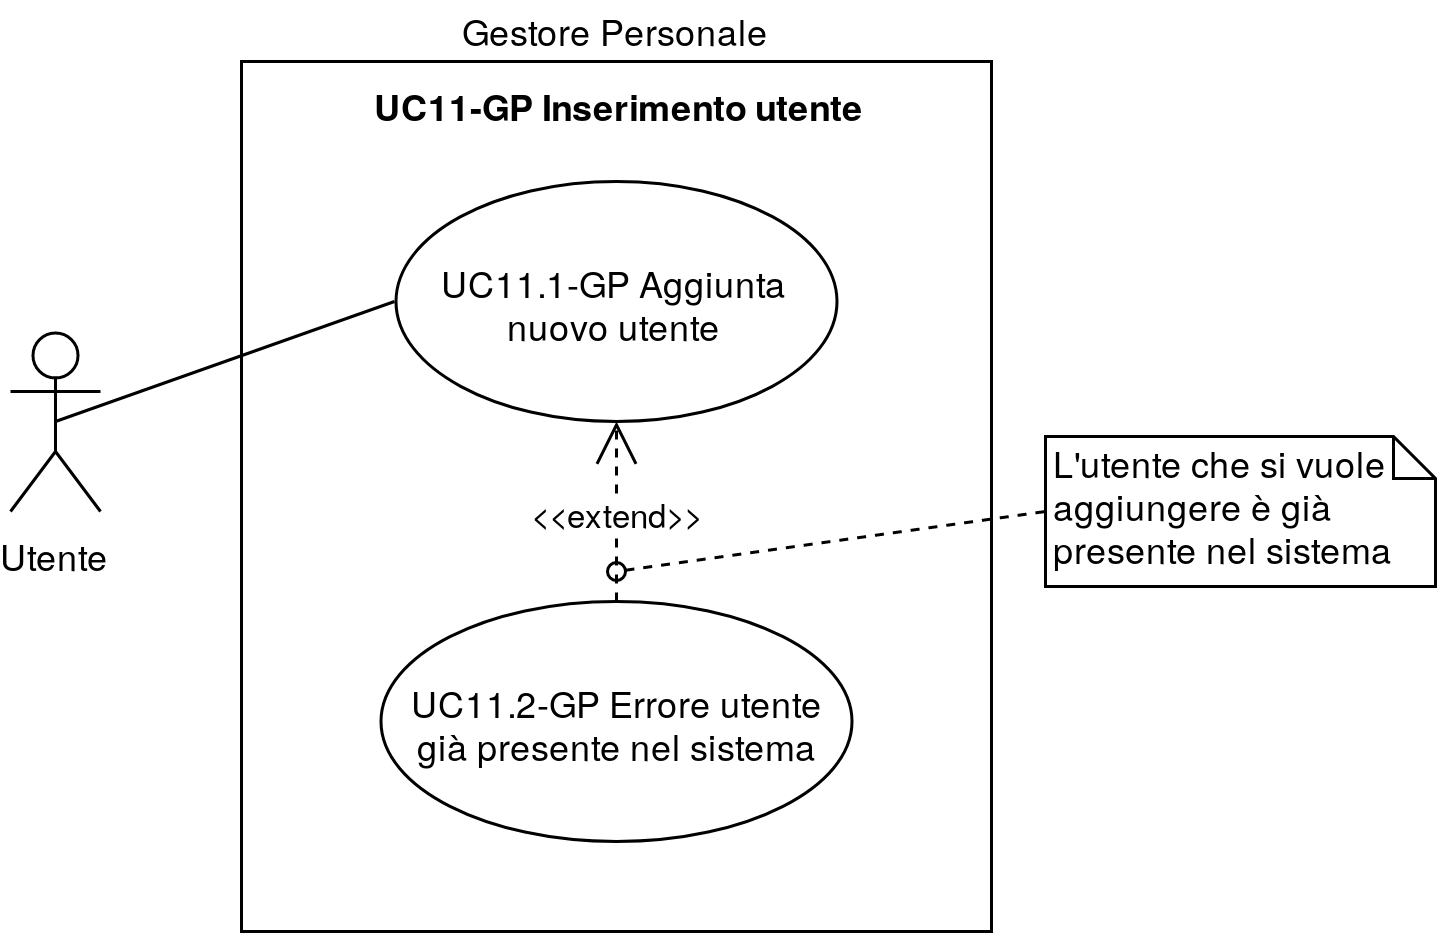
\includegraphics[width=0.8\textwidth]{img/casi_d'uso/UC11.png}\\
		\caption{UC\theuccount-BT - Consumer Telegram inoltra il messaggio finale al bot Telegram}
	\end{figure}
	\begin{itemize}
		\item \textbf{Codice}: UC\theuccount-BT.
		\item \textbf{Titolo}: Consumer Telegram inoltra il messaggio finale al bot Telegram.
		\item \textbf{Attori primari}: Consumer Telegram.
		\item \textbf{Descrizione}: il Consumer Telegram inoltra il messaggio finale al bot Telegram, il quale notifica il destinatario finale attraverso Telegram.
		\item \textbf{Precondizione}: il Consumer Telegram ha ricevuto almeno un messaggio.
		\item \textbf{Postcondizione}: il bot Telegram ha ricevuto il messaggio finale con successo.
		\item \textbf{Scenario principale}: 
		\begin{enumerate}
			\item Il Consumer Telegram riceve un messaggio dal Gestore Personale
			\item Il Consumer Telegram inoltra il messaggio finale al bot Telegram
		\end{enumerate}
		
	\end{itemize}